\documentclass[11pt,a4paper]{article}
\usepackage[utf8]{inputenc}
\usepackage[french]{babel}
\usepackage[T1]{fontenc}
\usepackage{amsmath}
\usepackage{amssymb}
\usepackage{graphicx}
\usepackage{geometry}
\usepackage{fancyhdr}
% \usepackage{circuitikz} % Décommenter si le package est disponible
% \usepackage{pgfplots} % Décommenter si le package est disponible
\usepackage{float}
% \pgfplotsset{compat=1.18} % Décommenter si le package est disponible

\geometry{margin=2cm}

% Configuration de l'en-tête
\pagestyle{fancy}
\fancyhf{} % Efface tous les en-têtes et pieds de page

% En-tête gauche
\fancyhead[L]{%
    \begin{tabular}[t]{@{}l@{}}
        \textbf{Nom:} KALIPE \\
        \textbf{Prénoms:} Kossi Mathias
    \end{tabular}%
}

% En-tête droite
\fancyhead[R]{%
    \begin{tabular}[t]{@{}l@{}}
        \textbf{}  \\
        \textbf{N° Étudiant:} 21507247
    \end{tabular}%
}

% Ligne horizontale sous l'en-tête
\renewcommand{\headrulewidth}{0.4pt}

% Pied de page (numéro de page centré)
\fancyfoot[C]{\thepage}

\title{\textbf{Préparation au TP\\Modulation d'Amplitude (Version Corrigée)}}
\author{Électronique des Systèmes Analogiques\\M1 SYSCOM | UM4EE101 - Sorbonne Université \\ \\ \textbf{N° Étudiant:} 21507247 \\ \textbf{Nom et prénoms:} KALIPE Kossi Mathias}

\date{}

\begin{document}

\maketitle

\section*{Introduction}

On désire transmettre par onde hertzienne un signal audio $S(t)$ dont le spectre s'étale sur une plage allant de 100 Hz à 3 kHz. La transmission directe de ce signal est impossible pour de nombreuses raisons :
\begin{itemize}
    \item Bruit important dans la bande basse fréquence
    \item Taille des antennes trop importante (longueur d'onde $\lambda = c/f$ trop grande)
    \item Mauvaise adaptation d'impédance des antennes dans cette bande
\end{itemize}

Il convient donc d'effectuer une modulation d'une porteuse $P(t)$ de fréquence $f_0$ fixe (bien supérieure à 3 kHz) par le signal $S(t)$.

\section{Modulation DSB (Double Side Band)}

\begin{figure}[H]
    \centering
    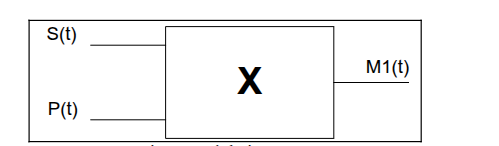
\includegraphics[width=0.8\linewidth]{../images/dsb.png}
    \caption{Circuit modulation DSB avec multiplieur analogique}
\end{figure}

\subsection{Question A.1 : Calcul de M1(t) et analyse spectrale}

\paragraph{Données}
\begin{itemize}
    \item Signal modulant : $S(t) = A_0 \cos(2\pi f_s t + \phi_s)$ avec $f_s < 3$ kHz
    \item Porteuse : $P(t) = B_0 \cos(2\pi f_0 t + \phi_0)$ avec $f_0 = 12$ kHz
    \item Signal modulé DSB : $M_1(t) = k \cdot S(t) \cdot P(t)$
\end{itemize}

\paragraph{Calcul de M1(t)}

En utilisant la formule de trigonométrie du produit de cosinus :
\begin{equation}
\cos(a) \cdot \cos(b) = \frac{1}{2}[\cos(a-b) + \cos(a+b)]
\end{equation}

On obtient :
\begin{align}
M_1(t) &= k \cdot A_0 \cos(2\pi f_s t + \phi_s) \cdot B_0 \cos(2\pi f_0 t + \phi_0) \\
&= \frac{k A_0 B_0}{2} [\cos(2\pi(f_0 - f_s)t + \phi_0 - \phi_s) + \cos(2\pi(f_0 + f_s)t + \phi_0 + \phi_s)]
\end{align}

\begin{equation}
\boxed{M_1(t) = \frac{k A_0 B_0}{2} [\cos(2\pi(f_0 - f_s)t + \Delta\phi_-) + \cos(2\pi(f_0 + f_s)t + \Delta\phi_+)]}
\end{equation}

avec $\Delta\phi_- = \phi_0 - \phi_s$ et $\Delta\phi_+ = \phi_0 + \phi_s$

\paragraph{Allure temporelle de M1(t)}

Le signal $M_1(t)$ est la somme de deux sinusoïdes de fréquences $(f_0 - f_s)$ et $(f_0 + f_s)$. Cette somme produit un phénomène de \textbf{battement}. L'enveloppe du signal varie à la fréquence $f_s$, et le signal s'annule (passage par zéro de l'enveloppe) deux fois par période de $S(t)$.

\paragraph{Indice de modulation}

Pour une modulation DSB pure (Double Side Band Suppressed Carrier), la notion classique d'indice de modulation $m$ (utilisée en AM, voir partie B) n'est \textbf{pas standardisée}. Le signal est simplement un produit. Il n'y a pas de porteuse résiduelle à laquelle comparer l'amplitude des bandes latérales.

\paragraph{Spectre de M1(t) pour $f_s = 1.5$ kHz}

Le spectre de $M_1(t)$ contient uniquement \textbf{deux raies spectrales} :

\begin{itemize}
    \item \textbf{Bande latérale inférieure (BLI)} : 
    \begin{equation}
    f_{BLI} = f_0 - f_s = 12 - 1.5 = 10.5 \text{ kHz}
    \end{equation}
    Amplitude : $\dfrac{k A_0 B_0}{2}$
    
    \item \textbf{Bande latérale supérieure (BLS)} : 
    \begin{equation}
    f_{BLS} = f_0 + f_s = 12 + 1.5 = 13.5 \text{ kHz}
    \end{equation}
    Amplitude : $\dfrac{k A_0 B_0}{2}$
\end{itemize}

\subsection{Question B.2 : Réalisation d'un modulateur AM}
\begin{figure}[H]
    \centering
    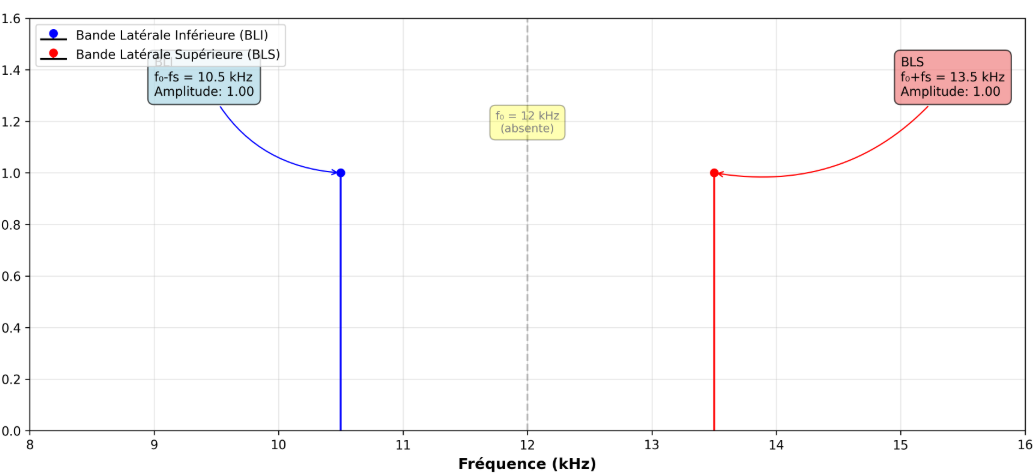
\includegraphics[width=0.8\linewidth]{../images/spectre_dsb.png}
    \caption{Spectre du signal modulé DSB $M_1(t)$}
\end{figure}

\textbf{Remarque cruciale :} La fréquence porteuse $f_0 = 12$ kHz \textbf{n'apparaît pas} dans le spectre. C'est la caractéristique "à porteuse supprimée" de la modulation DSB.

\paragraph{Cas d'une porteuse non sinusoïdale}

Si $P(t)$ est un signal périodique, il se décompose en série de Fourier (fondamentale $f_0$ + harmoniques $n f_0$) :
\begin{equation}
P(t) = \sum_{n=1}^{\infty} B_n \cos(2\pi n f_0 t + \phi_n)
\end{equation}

Le signal de sortie $M_1(t)$ devient :
\begin{equation}
M_1(t) \propto S(t) \cdot P(t) = \sum_{n=1}^{\infty} B_n \cos(2\pi n f_0 t + \phi_n) \cdot A_0 \cos(2\pi f_s t + \phi_s)
\end{equation}

\textbf{Conséquence sur le spectre :} Le spectre en sortie contient des bandes latérales $(n f_0 \pm f_s)$ autour de \textbf{toutes les harmoniques} de la porteuse. Cela crée une pollution spectrale importante et des interférences, rendant impératif l'usage d'une porteuse sinusoïdale pure.

\subsection{Question A.2 : Oscillateur à 12 kHz}

\paragraph{Analyse du circuit oscillateur (Fig. 2)}

Le circuit est un oscillateur à relaxation générant un signal triangulaire $V_2$, qui est ensuite filtré par le passe-bas $R_c C_c$ pour ne garder que la fondamentale sinusoïdale $V_3$.

\begin{enumerate}
    \item \textbf{Premier AOP (Comparateur à hystérésis)} : C'est un trigger de Schmitt. Sa sortie $V_1$ est un signal carré valant $\pm V_{sat} = \pm 10$ V. L'entrée du comparateur est $V_2$ (via $R_1$) et la réaction s'effectue via $R_2$. Le basculement se produit lorsque $V_2/R_1 = -V_1/R_2$.
    Les seuils de basculement en $V_2$ sont donc :
    \begin{equation}
    V_{seuil}^{\pm} = \mp V_{sat} \cdot \frac{R_1}{R_2}
    \end{equation}
    
    \item \textbf{Second AOP (Intégrateur inverseur)} : Il intègre le signal carré $V_1$ pour produire un signal triangulaire $V_2$. La pente de $V_2$ est constante et vaut :
    \begin{equation}
    \frac{dV_2}{dt} = -\frac{V_1}{RC} = \mp \frac{V_{sat}}{RC}
    \end{equation}
\end{enumerate}

\paragraph{Formes d'onde}
\begin{itemize}
    \item \textbf{En V1 :} Signal carré alternant entre $+10$ V et $-10$ V.
    \item \textbf{En V2 :} Signal triangulaire symétrique oscillant entre les seuils $+V_{sat} \frac{R_1}{R_2}$ et $-V_{sat} \frac{R_1}{R_2}$.
\end{itemize}

\paragraph{Expression de la fréquence d'oscillation}

Le temps d'une demi-période ($t_{1/2}$) est le temps pour $V_2$ de passer d'un seuil à l'autre.
\begin{equation}
t_{1/2} = \frac{\Delta V_2}{\text{pente}} = \frac{ (V_{sat} \frac{R_1}{R_2}) - (-V_{sat} \frac{R_1}{R_2}) }{V_{sat} / (RC)} = \frac{2 V_{sat} R_1 / R_2}{V_{sat} / RC} = 2 RC \frac{R_1}{R_2}
\end{equation}
La période $T = 2 \cdot t_{1/2} = 4 RC \frac{R_1}{R_2}$. La fréquence est donc :
\begin{equation}
\boxed{f_{osc} = \frac{1}{T} = \frac{R_2}{4 R_1 RC}}
\end{equation}
La fréquence dépend bien uniquement de $R_1, R_2, R$ et $C$.

\paragraph{Dimensionnement pour $f_{osc} = 12$ kHz et amplitude 10 V pp}

\textbf{Spécifications :}
\begin{itemize}
    \item Fréquence : $f_{osc} = 12$ kHz
    \item Sortie $V_3$ : 10 V pp (soit 5 V crête)
    \item Filtre : $R_c = 1.3$ k$\Omega$, $C_c = 10$ nF.
    Sa fréquence de coupure est $f_c = \frac{1}{2\pi R_c C_c} = \frac{1}{2\pi \cdot 1300 \cdot 10 \times 10^{-9}} \approx 12.24$ kHz.
\end{itemize}

\textbf{Étape 1 : Amplitude du signal triangulaire (V2)}
On veut $V_{3,crête} = 5$ V. $V_3$ est la sortie du filtre $R_c C_c$ dont l'entrée est $V_2$.
Le gain du filtre à $f_{osc}=12$ kHz est $G = \frac{1}{\sqrt{1+(f_{osc}/f_c)^2}} = \frac{1}{\sqrt{1+(12/12.24)^2}} \approx 0.715$.
$V_3$ est la fondamentale de $V_2$ (triangulaire), atténuée par $G$.
$V_{3,crête} = V_{2,fond} \times G$.
Donc, l'amplitude de la fondamentale de $V_2$ doit être $V_{2,fond} = 5 \text{ V} / 0.715 \approx 7.0$ V (crête).
Pour un triangle, $V_{fond} = V_{crête} \times \frac{8}{\pi^2}$.
L'amplitude crête du triangle $V_2$ doit donc être $V_{2,crête} = V_{2,fond} \times \frac{\pi^2}{8} \approx 7.0 \times 1.234 \approx 8.64$ V.
On sait que $V_{2,crête} = V_{seuil}^+ = V_{sat} \frac{R_1}{R_2} = 10 \frac{R_1}{R_2}$.
$8.64 = 10 \frac{R_1}{R_2} \implies \frac{R_2}{R_1} = \frac{10}{8.64} \approx 1.157$.
Choisissons des valeurs normalisées : $\boxed{R_1 = 10 \text{ k}\Omega, \quad R_2 = 12 \text{ k}\Omega}$.

\textbf{Étape 2 : Calcul de R et C}
On utilise la formule de fréquence : $f_{osc} = \frac{R_2}{4 R_1 RC} \implies RC = \frac{R_2}{4 R_1 f_{osc}}$.
\begin{equation}
RC = \frac{12 \times 10^3}{4 \times (10 \times 10^3) \times 12000} = \frac{12 \times 10^3}{480 \times 10^6} = 2.5 \times 10^{-5} \text{ s}
\end{equation}
Choisissons une valeur standard : $\boxed{C = 10 \text{ nF}}$ (valeur plausible, $C_c$ vaut 10nF).
\begin{equation}
R = \frac{2.5 \times 10^{-5}}{10 \times 10^{-9}} = 2500 \, \Omega
\end{equation}
Valeur normalisée : $\boxed{R = 2.4 \text{ k}\Omega}$ (ou $2.7$ k$\Omega$).
Avec $R=2.4$ k$\Omega$, $f_{osc} = \frac{12k}{4 \cdot 10k \cdot 2.4k \cdot 10n} = 12.5$ kHz, ce qui est très proche.

\subsection{Question A.3 : Multiplication avec le circuit AD633}

\paragraph{Fonction du circuit AD633}
Le multiplieur réalise $V_{out} = \frac{(X_1 - X_0)(Y_1 - Y_0)}{10\text{ V}} + Z$.

\paragraph{Plan de câblage pour obtenir $M_1(t) = S(t) \cdot P(t) / 10$}

\textbf{Objectif :} Réaliser la modulation DSB $M_1(t) = \dfrac{S(t) \cdot P(t)}{10}$.
\textbf{Connexions proposées :}
\begin{itemize}
    \item $X_1$ : Signal modulant $S(t)$ du GBF (10 V pp, 1.5 kHz)
    \item $X_0$ : Masse (0 V)
    \item $Y_1$ : Porteuse $P(t)$ (point $V_3$ de l'oscillateur, 10 V pp, 12 kHz)
    \item $Y_0$ : Masse (0 V)
    \item $Z$ : Masse (0 V)
    \item $V_{CC+}$ : +12 V (alimentation positive)
    \item $V_{CC-}$ : -12 V (alimentation négative)
    \item $out$ : Signal modulé $M_1(t)$
\end{itemize}
Avec ce câblage, on obtient : $V_{out} = \frac{(S(t) - 0)(P(t) - 0)}{10} + 0$, soit le résultat désiré.

\paragraph{Analyse de la démodulation DSB}
La démodulation (dite synchrone) nécessite de multiplier $M_1(t)$ par une porteuse locale $P_L(t)$ parfaitement en phase et en fréquence avec la porteuse d'émission.
Comme calculé dans le document, après filtrage passe-bas, on récupère un terme proportionnel à $S(t)$.
\textbf{Inconvénient majeur :} Le signal DSB $M_1(t)$ ne contient pas la fréquence porteuse $f_0$. Le récepteur doit donc posséder un oscillateur local complexe synchronisé (PLL, boucle de Costas) pour recréer $P_L(t)$, ce qui est un inconvénient majeur.

\section{Modulation AM (Amplitude Modulation)}

\begin{figure}[H]
    \centering
    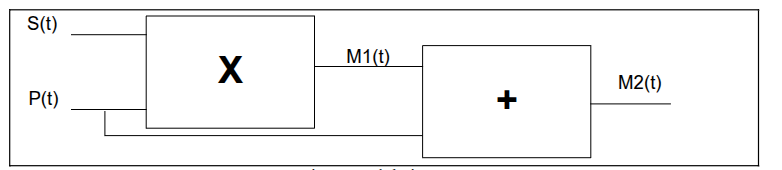
\includegraphics[width=0.8\linewidth]{../images/am.png}
    \caption{Circuit modulation AM avec addition de porteuse}
\end{figure}

\subsection{Question B.1 : Calcul de M2(t) et analyse}

\paragraph{Principe de la modulation AM}
Pour éviter le problème de reconstitution de porteuse, on l'ajoute au signal émis (Fig. 4) :
\begin{equation}
M_2(t) = P(t) + M_1(t) = P(t) + k \cdot S(t) \cdot P(t) = P(t)[1 + k \cdot S(t)]
\end{equation}

\paragraph{Expression mathématique de M2(t)}
Avec $S(t) = A_0 \cos(2\pi f_s t)$ et $P(t) = B_0 \cos(2\pi f_0 t)$ :
\begin{equation}
M_2(t) = B_0 \cos(2\pi f_0 t) \cdot [1 + k A_0 \cos(2\pi f_s t)]
\end{equation}
On pose $\boxed{m = k A_0}$ comme étant l'indice de modulation.
\begin{equation}
\boxed{M_2(t) = B_0[1 + m \cos(2\pi f_s t)] \cos(2\pi f_0 t)}
\end{equation}

\paragraph{Indice de modulation}
L'amplitude instantanée (l'enveloppe) de $M_2(t)$ varie entre :
\begin{itemize}
    \item Amplitude maximale : $A_{max} = B_0(1 + m)$
    \item Amplitude minimale : $A_{min} = B_0(1 - m)$
\end{itemize}
L'indice de modulation se mesure sur l'oscilloscope par :
$m = \frac{A_{max} - A_{min}}{A_{max} + A_{min}}$.

\paragraph{Allure temporelle pour différents indices de modulation}

\textbf{Cas 1 : $m = 0.5$ (sous-modulation)}
\begin{itemize}
    \item L'enveloppe varie entre $0.5 B_0$ et $1.5 B_0$. Elle ne s'annule jamais.
    \item L'enveloppe reproduit fidèlement $S(t)$. Démodulation par détection d'enveloppe possible.
\end{itemize}

\textbf{Cas 2 : $m = 1$ (modulation à 100\%)}
\begin{itemize}
    \item L'enveloppe varie entre $0$ et $2 B_0$.
    \item Cas limite pour la détection d'enveloppe. Puissance maximale dans les bandes latérales.
\end{itemize}

\textbf{Cas 3 : $m = 2$ (surmodulation)}
\begin{itemize}
    \item L'enveloppe "devrait" varier entre $-B_0$ et $3 B_0$.
    \item Le passage par une amplitude négative provoque un \textbf{renversement de phase} de la porteuse.
    \item L'enveloppe est distordue (redressement). $S(t)$ n'est plus récupérable par un simple détecteur d'enveloppe.
\end{itemize}

\paragraph{Spectres de M2(t)}
En développant l'expression de $M_2(t)$ :
\begin{align}
M_2(t) &= B_0\cos(2\pi f_0 t) + m B_0 \cos(2\pi f_s t) \cos(2\pi f_0 t) \\
&= \underbrace{B_0\cos(2\pi f_0 t)}_{\text{Porteuse}} + \underbrace{\frac{m B_0}{2}[\cos(2\pi(f_0-f_s)t) + \cos(2\pi(f_0+f_s)t)]}_{\text{Bandes latérales (BLI + BLS)}}
\end{align}
Le spectre contient \textbf{trois raies} (pour $f_s=1.5$ kHz) :
\begin{itemize}
    \item \textbf{Porteuse} : $f = f_0 = 12$ kHz, amplitude $B_0$
    \item \textbf{BLI} : $f = f_0 - f_s = 10.5$ kHz, amplitude $\dfrac{m B_0}{2}$
    \item \textbf{BLS} : $f = f_0 + f_s = 13.5$ kHz, amplitude $\dfrac{m B_0}{2}$
\end{itemize}


\begin{figure}[H]
    \centering
    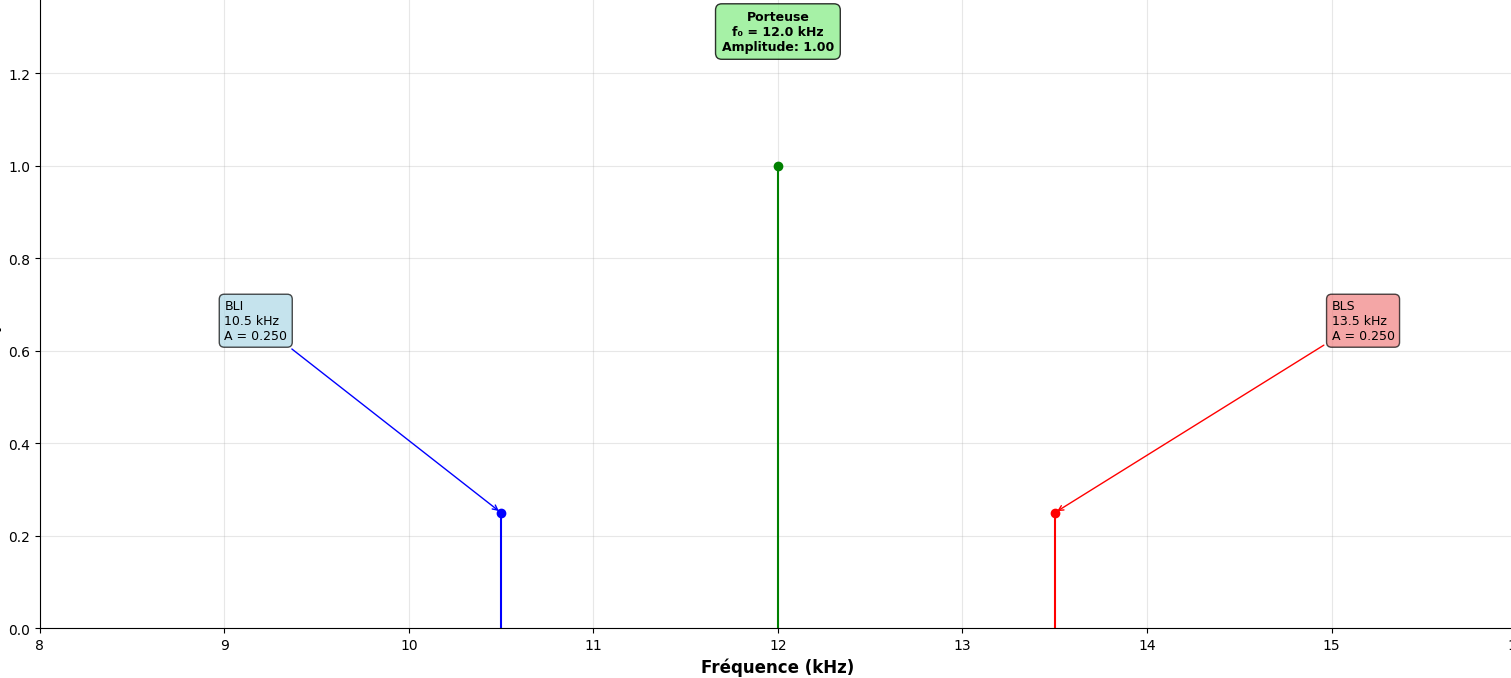
\includegraphics[width=0.8\linewidth]{../images/spectre_am_05.png}
    \caption{Spectre du signal modulé AM $M_2(t)$ pour $m=0.5$}
\end{figure}
\begin{figure}[H]
    \centering
    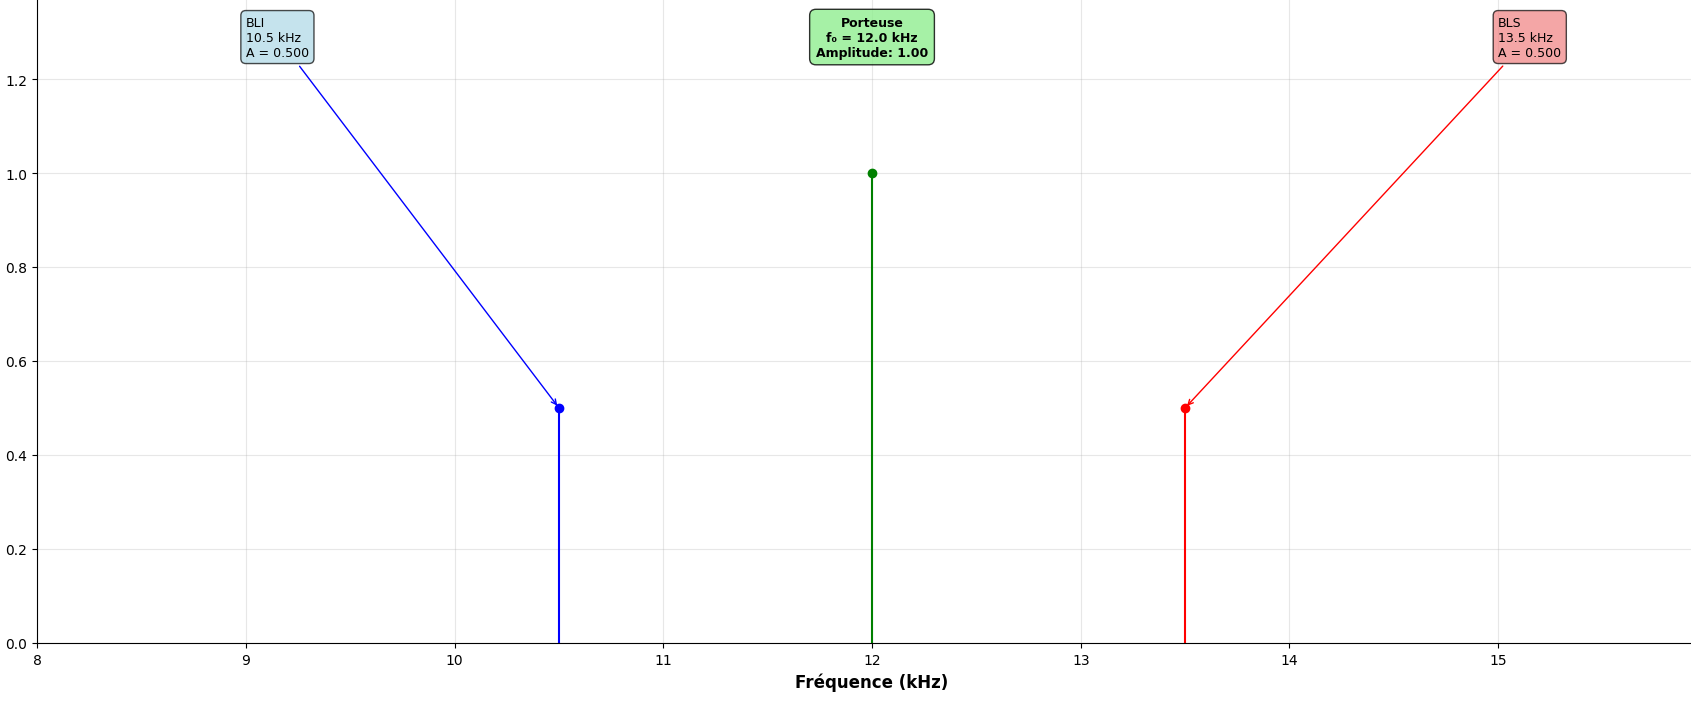
\includegraphics[width=0.8\linewidth]{../images/spectre_am1.png}
    \caption{Spectre du signal modulé AM $M_2(t)$ pour $m=1$}
\end{figure}
\begin{figure}[H]
    \centering
    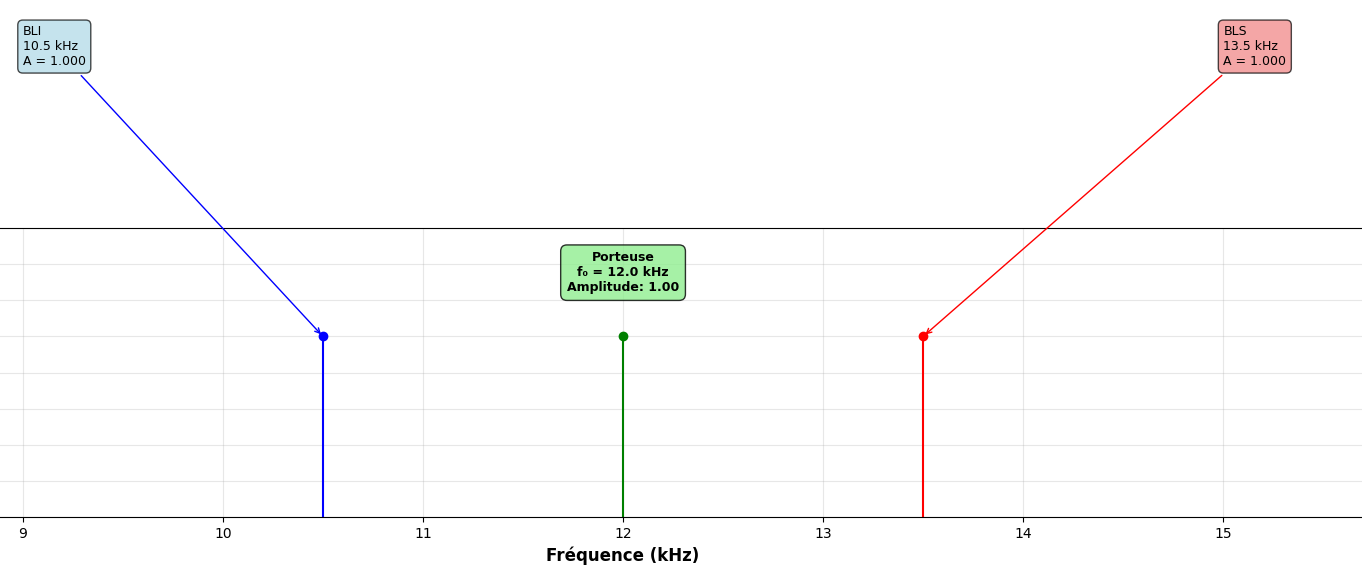
\includegraphics[width=0.8\linewidth]{../images/spectre_am_2.png}
    \caption{Spectre du signal modulé AM $M_2(t)$ pour $m=2$}
\end{figure}


Contrairement à la DSB, la porteuse est présente, transportant la référence de phase et de fréquence.

\subsection{Question B.2 : Réalisation d'un modulateur AM}
\begin{figure}[H]
    \centering
    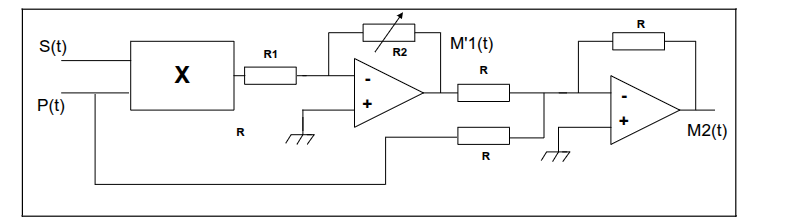
\includegraphics[width=0.8\linewidth]{../images/am_realisation.png}
    \caption{Circuit modulateur AM avec multiplieur et sommateur}
\end{figure}

\paragraph{Analyse du montage de la figure 3}
Le montage utilise le multiplieur AD633 pour générer le terme DSB, puis un sommateur inverseur pour ajouter la porteuse.
\begin{itemize}
    \item Multiplieur (X) : Sort $S(t)P(t)/10$.
    \item AOP (sommateur) : $M_2(t) = - \left( \frac{R_2}{R_1} \left[ \frac{S(t)P(t)}{10} \right] + \frac{R_2}{R} P(t) \right)$
\end{itemize}
Sur la Fig. 3, les résistances d'entrée du sommateur sont $R_1$ et $R$.
En posant $R = R_1$ (ce qui est visuellement le cas sur le schéma) :
\begin{equation}
M_2(t) = -\frac{R_2}{R_1} \left( \frac{S(t)P(t)}{10} + P(t) \right) = -\frac{R_2}{R_1} P(t) \left[ 1 + \frac{S(t)}{10} \right]
\end{equation}
Le signe 'moins' est une simple inversion de phase, sans impact sur l'enveloppe.

\paragraph{Gain maximal sans saturation}
\textbf{Données :}
\begin{itemize}
    \item Amplitudes d'entrée : $S(t)$ et $P(t)$ : 10 V pp $\Rightarrow$ 5 V crête.
    \item Tensions de saturation des AOP TL081 : $\pm 10$ V.
\end{itemize}
D'après l'expression $M_2(t)$ ci-dessus, l'indice de modulation est fixé par $S(t)$:
\begin{equation}
m = \frac{S(t)_{crête}}{10} = \frac{5 \text{ V}}{10} = 0.5
\end{equation}
Le potentiomètre $R_2$ (variable) ajuste le gain global $G = R_2/R_1$, mais pas l'indice $m$.
L'amplitude maximale de la sortie $M_2(t)$ est :
\begin{equation}
|M_2(t)|_{max} = G \cdot P(t)_{crête} \cdot (1 + m)
\end{equation}
\begin{equation}
|M_2(t)|_{max} = G \cdot 5 \text{ V} \cdot (1 + 0.5) = G \cdot 7.5 \text{ V}
\end{equation}
Pour éviter la saturation à $\pm 10$ V :
\begin{equation}
G \cdot 7.5 \text{ V} \leq 10 \text{ V} \implies \boxed{G_{max} = \frac{10}{7.5} \approx 1.33}
\end{equation}
Le gain maximal $R_2/R_1$ doit être d'environ 1.33 pour ne pas saturer.

\paragraph{Expression de l'indice de modulation}
Comme calculé ci-dessus, en supposant $R_1=R$ (comme sur le schéma Fig. 7) :
\begin{equation}
\boxed{m = \frac{S(t)_{crête}}{10}}
\end{equation}
Avec $S(t)_{crête} = 5$ V, l'indice est fixé à $m=0.5$.

\section{Démodulation}
\begin{figure}[H]
    \centering
    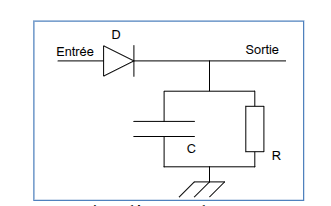
\includegraphics[width=0.8\linewidth]{../images/crete.png}
    \caption{Circuit détecteur de crête pour démodulation AM}
\end{figure}

\subsection{Question C.1 : Démodulation par détection d'enveloppe}

\paragraph{Principe de la détection d'enveloppe}
Consiste à extraire l'enveloppe $B_0[1 + m \cos(2\pi f_s t)]$ du signal modulé AM pour retrouver le signal modulant $S(t)$.

\paragraph{Condition sur l'indice de modulation}
La détection d'enveloppe ne fonctionne correctement que si l'enveloppe ne s'annule jamais (pas de surmodulation).
\begin{equation}
\boxed{m \leq 1}
\end{equation}
Si $m > 1$, l'enveloppe est distordue par le renversement de phase, et le signal démodulé n'est plus $S(t)$.

\paragraph{Principe du détecteur de crête (Fig. 8)}
\begin{itemize}
    \item \textbf{Diode D} : Redresse le signal (charge le condensateur lors des crêtes positives).
    \item \textbf{Condensateur C} : Se charge rapidement aux crêtes $\approx A_{max}$.
    \item \textbf{Résistance R} : Permet la décharge lente du condensateur pour suivre l'enveloppe.
\end{itemize}

\paragraph{Choix de la constante de temps RC}
La constante $\tau = RC$ doit satisfaire deux conditions contradictoires :

\textbf{Condition 1 : Filtrer la porteuse}
Le condensateur doit se décharger très peu entre deux crêtes de la porteuse.
\begin{equation}
\tau \gg T_0 = \frac{1}{f_0} = \frac{1}{12000} = 83.3 \, \mu\text{s}
\end{equation}

\textbf{Condition 2 : Suivre les variations du signal modulant}
Le condensateur doit pouvoir se décharger assez vite pour suivre la pente descendante de l'enveloppe, surtout à la fréquence $f_{s,max} = 3$ kHz. La condition stricte pour éviter la distorsion diagonale est :
\begin{equation}
\tau \leq \frac{\sqrt{1-m^2}}{m \cdot 2\pi f_{s,max}}
\end{equation}

\textbf{Contradiction et compromis :}
Dans le cas le pire ($f_s = 3$ kHz et $m$ proche de 1) :
\begin{equation}
\tau \leq \frac{\sqrt{1-0.95^2}}{0.95 \cdot 2\pi \cdot 3000} \approx 17.5 \, \mu\text{s}
\end{equation}
Nous avons une \textbf{contradiction insoluble} : $\tau$ doit être $\gg 83.3 \, \mu\text{s}$ et $\leq 17.5 \, \mu\text{s}$.
\textbf{Conclusion :} La détection d'enveloppe simple \textbf{ne peut pas fonctionner} sans distorsion pour ce signal lorsque $f_s$ est élevée (3 kHz) et $m$ est proche de 1.
Un compromis (ex: $\tau = 100 \, \mu\text{s}$) filtrera la porteuse mais introduira une distorsion diagonale sévère aux hautes fréquences du signal modulant.

\subsection{Question C.2 : Démodulation par produit}

\paragraph{Principe}
Aussi appelée démodulation synchrone. Consiste à multiplier le signal modulé ($M_1$ ou $M_2$) par la porteuse $P(t)$, puis à filtrer en passe-bas.

\paragraph{Produit D1(t) = M1(t) · P(t) (DSB)}
Rappel : $M_1(t) = \frac{k A_0 B_0}{2}[\cos(2\pi(f_0-f_s)t) + \cos(2\pi(f_0+f_s)t)]$
En multipliant par $P(t) = B_0 \cos(2\pi f_0 t)$ et en utilisant $\cos(a)\cos(b) = \frac{1}{2}[\cos(a-b) + \cos(a+b)]$ :
\begin{align}
D_1(t) = \frac{k A_0 B_0^2}{4} [&\cos(2\pi f_s t) + \cos(2\pi(2f_0-f_s)t) \\
&+ \cos(2\pi f_s t) + \cos(2\pi(2f_0+f_s)t)]
\end{align}
\begin{equation}
\boxed{D_1(t) = \underbrace{\frac{k A_0 B_0^2}{2} \cos(2\pi f_s t)}_{\text{Terme utile (Signal)}} + \underbrace{\frac{k A_0 B_0^2}{4}[\cos(2\pi(2f_0-f_s)t) + \cos(2\pi(2f_0+f_s)t)]}_{\text{Termes Haute Fréquence}}}
\end{equation}

\paragraph{Produit D2(t) = M2(t) · P(t) (AM)}
Avec $M_2(t) = B_0[1 + m \cos(2\pi f_s t)] \cos(2\pi f_0 t)$ et $m=kA_0$ :
\begin{align}
D_2(t) &= B_0[1 + k A_0 \cos(2\pi f_s t)] \cos(2\pi f_0 t) \times B_0 \cos(2\pi f_0 t) \\
&= B_0^2[1 + k A_0 \cos(2\pi f_s t)] \cos^2(2\pi f_0 t)
\end{align}
En utilisant $\cos^2(x) = \dfrac{1 + \cos(2x)}{2}$ :
\begin{equation}
D_2(t) = \frac{B_0^2}{2}[1 + k A_0 \cos(2\pi f_s t)][1 + \cos(4\pi f_0 t)]
\end{equation}
En développant :
\begin{align}
D_2(t) = \frac{B_0^2}{2} + \frac{k A_0 B_0^2}{2}\cos(2\pi f_s t) + \text{termes HF (autour de } 2f_0\text{)}
\end{align}
\begin{equation}
\boxed{D_2(t) = \underbrace{\frac{B_0^2}{2}}_{\text{DC}} + \underbrace{\frac{k A_0 B_0^2}{2}\cos(2\pi f_s t)}_{\text{Terme utile (Signal)}} + \underbrace{\text{Termes HF à } 2f_0 \text{ et } 2f_0 \pm f_s}_{\text{Termes Haute Fréquence}}}
\end{equation}

\paragraph{Fréquences des termes parasites}
Dans les deux cas, le filtrage passe-bas doit éliminer :
\begin{itemize}
    \item \textbf{Composante continue} : 0 Hz (uniquement pour $D_2$)
    \item \textbf{Bandes autour de $2f_0$} : $2f_0 - f_s = 22.5$ kHz et $2f_0 + f_s = 25.5$ kHz.
\end{itemize}
Toutes ces fréquences (sauf DC) sont bien au-delà de la bande utile (100 Hz - 3 kHz).

\paragraph{Avantages de la démodulation par produit}
Elle fonctionne parfaitement quel que soit l'indice de modulation (même $m > 1$) et n'introduit pas de distorsion diagonale. Elle nécessite cependant une porteuse locale synchrone (ce qui, pour $M_2$, peut être obtenu en filtrant la porteuse de $M_2$).

\subsection{Question C.3 : Filtrage}
\begin{figure}[H]
    \centering
    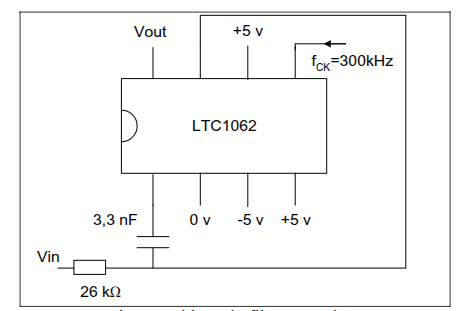
\includegraphics[width=0.8\linewidth]{../images/pass_bas.png}
    \caption{Filtre passe-bas LTC1062 pour démodulation par produit}
\end{figure}
\begin{figure}[H]
    \centering
    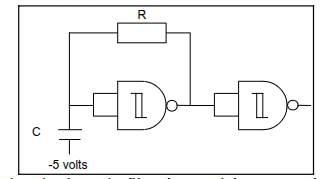
\includegraphics[width=0.8\linewidth]{../images/horloge.png}
    \caption{Génération de l'horloge pour le filtre LTC1062}
\end{figure}

\paragraph{Principe du filtrage}
On utilise un filtre passe-bas pour ne conserver que le terme utile (100 Hz - 3 kHz) et supprimer les composantes DC et HF ($> 22.5$ kHz).

\paragraph{Filtre LTC1062}
C'est un filtre à capacités commutées, configuré en Butterworth d'ordre 5. Sa fréquence de coupure $f_c$ est déterminée par l'horloge $f_{CK}$ :
\begin{equation}
f_c = \frac{f_{CK}}{100}
\end{equation}
Pour une $f_c$ désirée de 3 kHz (limite haute de $S(t)$) :
\begin{equation}
\boxed{f_{CK} = 100 \times f_c = 100 \times 3000 = 300 \text{ kHz}}
\end{equation}
C'est bien la valeur $f_{CK}=300$ kHz indiquée sur la Fig. 9.

\paragraph{Génération de l'horloge (Figure 10)}
L'oscillateur (CD4093) génère un signal carré. La formule de fréquence pour cet oscillateur (relaxateur à porte NAND Trigger) est $f \approx \frac{1}{k RC}$. Le facteur $k$ dépend du type de porte (pour un CD4093, $k \approx 2.2$ n'est pas standard, $k \approx 1/0.6$ est plus courant, mais suivons le TP). Si $f = 1/(2.2 RC)$ :
\begin{equation}
RC = \frac{1}{2.2 \times f_{CK}} = \frac{1}{2.2 \times 300000} \approx 1.515 \times 10^{-6} \text{ s}
\end{equation}
\textbf{Choix des composants:}
Si on choisit $\boxed{C = 1 \text{ nF}}$ :
\begin{equation}
R = \frac{1.515 \times 10^{-6}}{1 \times 10^{-9}} = 1515 \, \Omega \implies \text{Standard } \boxed{R = 1.5 \text{ k}\Omega}
\end{equation}

\paragraph{Atténuation des termes parasites}
Le filtre est un Butterworth d'ordre 5.
Sa pente d'atténuation en dehors de la bande passante est de $n \times (-20 \text{ dB/décade})$ :
\begin{equation}
\text{Pente} = 5 \times (-20 \text{ dB/décade}) = \mathbf{-100} \text{ dB/décade}
\end{equation}
L'atténuation $A$ (en dB) pour $f \gg f_c$ est $A(f) \approx -100 \log_{10}\left(\frac{f}{f_c}\right)$.

Les premiers termes parasites sont à $f_{parasite} \approx 22.5$ kHz.
\begin{equation}
\frac{f_{parasite}}{f_c} = \frac{22.5 \text{ kHz}}{3 \text{ kHz}} = 7.5
\end{equation}
\begin{equation}
A_{dB} \approx -100 \times \log_{10}(7.5) \approx -100 \times 0.875 \approx \mathbf{-87.5 \text{ dB}}
\end{equation}
Cela correspond à une atténuation d'amplitude d'un facteur $10^{-87.5/20} \approx 4.2 \times 10^{-5}$.


\textbf{Conclusion :} Les termes haute fréquence sont très efficacement supprimés, et le signal $S(t)$ est récupéré avec une grande pureté.

\vspace{1cm}

\end{document}